%% FullCourse_10Lecs -- Lecture 8, Topic 8.4a: Augmented Generation + RAG vs Fine-Tune + Applications
%% Source: Phase 1 split from ./archive_pre_split/Lec08_T4_Augmented_Gen_Apps_Wrap.tex
%%   T4 was split at the demo boundary: T4a holds Sections I-III + closing Synthesis;
%%   T4b holds the OLG demo, failure modes, evaluation, and the Lec09 bridge.

%% Shared preamble for the FullCourse_10Lecs topic decks.
%%
%% Each topic .tex \input's this file, then defines its own \title, \date
%% override (if any), \graphicspath, and \begin{document}.
%%
%% Reconstructed verbatim from the inlined copy preserved in
%% Lec10_Case_Studies/Lec10_T8_Case6_DeepRamsey.tex (lines 23-190), which is
%% explicitly annotated there as "from ../shared_preamble.tex, copied verbatim".
%% Base preamble matches MiniCourse_8hr/Slides/shared_preamble.tex; this version
%% additionally provides \sectiondivider, the conceptbox/cautionbox/examplebox/
%% takeawaybox tcolorboxes, and \compacttables used across the split decks.

\documentclass[10pt,english,aspectratio=169]{beamer}

\usepackage{ae,aecompl}
\usepackage[T1]{fontenc}
\usepackage{textcomp}
\usepackage[utf8]{inputenc}
\usepackage{babel}
\usepackage{datetime2}

\setcounter{secnumdepth}{3}
\setcounter{tocdepth}{3}

\usepackage{amsmath, amssymb, amsthm, graphicx}
\usepackage{booktabs, multirow}
\usepackage{tikz}
\usepackage{pgfplots}
\pgfplotsset{compat=1.16}
\usepackage[most]{tcolorbox}
\tcbuselibrary{skins, breakable, theorems}
\usepackage{listings}
\usepackage{xcolor}

\lstset{
  basicstyle=\ttfamily\small,
  keywordstyle=\color{blue!80!black}\bfseries,
  commentstyle=\color{green!50!black}\itshape,
  stringstyle=\color{orange!80!black},
  backgroundcolor=\color{gray!8},
  frame=single,
  rulecolor=\color{gray!40},
  breaklines=true,
  showstringspaces=false,
  numbers=none,
}

\lstdefinestyle{pythonstyle}{
    language=Python,
    basicstyle=\ttfamily\footnotesize,
    keywordstyle=\color{blue!80!black}\bfseries,
    commentstyle=\color{green!50!black}\itshape,
    stringstyle=\color{orange!80!black},
    frame=single,
    breaklines=true,
    showstringspaces=false,
    numbers=left,
    numbersep=5pt,
    numberstyle=\tiny\color{gray},
    backgroundcolor=\color{gray!8},
    rulecolor=\color{gray!40}
}

\ifx\hypersetup\undefined
  \AtBeginDocument{%
    \hypersetup{bookmarks=false,breaklinks=true,pdfborder={0 0 0},colorlinks=true,
      linkcolor=DarkText,urlcolor=RedTitle}%
  }
\else
  \hypersetup{bookmarks=false,breaklinks=true,pdfborder={0 0 0},colorlinks=true,
    linkcolor=DarkText,urlcolor=RedTitle}%
\fi

\makeatletter
\newcommand\makebeamertitle{%
  \begin{frame}[plain]
    \vspace*{1.0cm}
    \centering
    {\usebeamerfont{title}\usebeamercolor[fg]{title}\inserttitle\par}
    \vspace{1.0cm}
    {\usebeamerfont{author}\usebeamercolor[fg]{author}\insertauthor\par}
    \vspace{0.2cm}
    {\usebeamerfont{date}\usebeamercolor[fg]{date}\insertdate\par}
  \end{frame}}%
\AtBeginDocument{%
  \let\origtableofcontents=\tableofcontents
  \def\tableofcontents{\@ifnextchar[{\origtableofcontents}{\gobbletableofcontents}}
  \def\gobbletableofcontents#1{\origtableofcontents}%
}

\usetheme{metropolis}
\usefonttheme{professionalfonts}

\definecolor{LightGray}{RGB}{230,230,230}
\definecolor{RedTitle}{RGB}{0,0,200}
\definecolor{VeryLightGray}{RGB}{245,245,245}
\definecolor{DarkText}{RGB}{0,0,0}

\setbeamercolor{background canvas}{bg=white}
\setbeamercolor{title}{fg=RedTitle}
\setbeamercolor{author}{fg=DarkText}
\setbeamercolor{date}{fg=DarkText}
\setbeamercolor{frametitle}{bg=VeryLightGray,fg=DarkText}
\setbeamercolor{normal text}{fg=DarkText}
\setbeamerfont{title}{size=\large}

\setbeamersize{text margin left=5mm, text margin right=5mm}
\addtobeamertemplate{frametitle}{}{\vspace{-0.5em}}
\newcommand{\reducevspace}{\vspace{-0.5cm}}

% Shared section divider and box styles for split topic decks.
\newcommand{\sectiondivider}[2]{%
\begin{frame}[plain,noframenumbering]
\begin{center}
\vfill
{\Large\textbf{#1}\par}
\vspace{0.35cm}
{\normalsize #2\par}
\vfill
\end{center}
\end{frame}
}

\newtcolorbox{conceptbox}[1][]{
  colback=blue!3,
  colframe=RedTitle!55,
  boxrule=0.35mm,
  arc=1mm,
  left=2mm,
  right=2mm,
  top=1mm,
  bottom=1mm,
  #1
}
\newtcolorbox{cautionbox}[1][]{
  colback=red!3,
  colframe=red!50!black,
  boxrule=0.35mm,
  arc=1mm,
  left=2mm,
  right=2mm,
  top=1mm,
  bottom=1mm,
  #1
}
\newtcolorbox{examplebox}[1][]{
  colback=green!3,
  colframe=green!45!black,
  boxrule=0.35mm,
  arc=1mm,
  left=2mm,
  right=2mm,
  top=1mm,
  bottom=1mm,
  #1
}
\newtcolorbox{takeawaybox}[1][]{
  colback=VeryLightGray,
  colframe=RedTitle!55,
  boxrule=0.35mm,
  arc=1mm,
  left=2mm,
  right=2mm,
  top=1mm,
  bottom=1mm,
  #1
}
\newcommand{\compacttables}{\renewcommand{\arraystretch}{1.15}}

\setbeamertemplate{navigation symbols}{}
\setbeamertemplate{footline}{%
  \hfill%
  \usebeamercolor[fg]{page number in head/foot}%
  \usebeamerfont{page number in head/foot}%
  \insertframenumber\,/\,\inserttotalframenumber\kern1em\vskip2pt%
}

\makeatother

\author{Zhigang Feng}
% "date with time": compile timestamp so each build is identifiable.
\date{\today\ \DTMcurrenttime}


% colortbl for \cellcolor in the RAG vs FT decision matrix
\usepackage{colortbl}

\usetikzlibrary{arrows.meta, positioning, shapes.geometric, fit, calc, backgrounds}

\graphicspath{{./pic/}{./figures/}{../../MiniCourse_8hr/Slides/Module4_Agentic_AI/pic/}{../}}

\title[AI for Econ Research]{AI for Economic Research: Dynamic Models, Language, and Agents\\
Lecture 8.4a: Augmented Generation, RAG vs Fine-Tuning, Applications}

\begin{document}

\makebeamertitle

%=============================================================================
\begin{frame}{Topic 8.4a Agenda}
\begin{enumerate}
  \item \textbf{Augmented Generation}
  \medskip
  \item \textbf{RAG vs Fine-Tuning}
  \medskip
  \item \textbf{Economic Applications}
  \medskip
  \item \textbf{Synthesis: Three Workflow Patterns}
\end{enumerate}

\medskip
\textit{Arc: T1 Prompting wall $\to$ T2 Chunking \& embeddings $\to$ T3 Vector \& graph retrieval $\to$ \textbf{T4a Augmented generation} $\to$ T4b Demo, failures, agentic bridge}
\end{frame}

%=============================================================================
\section{Augmented Generation}

\begin{frame}{From Retrieved Chunks to a Final Answer}
\begin{itemize}
\item We now have the top-$K$ chunks for the user's query (typically $K = 3$ to $10$). What do we do with them?

\medskip
\item \textbf{Insert them into a prompt template, send to the LLM.} The model sees:
\begin{enumerate}
    \item System instructions (how to behave)
    \item The retrieved chunks (the evidence)
    \item The user question
    \item Output-format instructions (how to cite)
\end{enumerate}

\medskip
\item The LLM now \textbf{generates} an answer that is \emph{grounded in the retrieved evidence}.

\medskip
\item This is the only place a generative model is used in the whole pipeline. Everything before this --- chunking, embedding, retrieval --- exists to put high-quality evidence in front of the model.

\medskip
\item \textbf{The single most important design choice} at this stage: the \emph{prompt template}.
\end{itemize}
\end{frame}

\begin{frame}[fragile]{Prompt Template --- Anatomy}
A real RAG prompt has four parts. Lines below are color-coded by role:
\begin{lstlisting}
SYSTEM:
You are a research assistant for academic economists.
Answer the user's question using ONLY the context below.
If the context does not contain the answer, reply
exactly: "I don't know based on the provided sources."
Cite sources inline using [doc_id:page] notation.

CONTEXT:
[1] (fomc_2024_06:p3)
"Participants observed that inflation remained elevated..."

[2] (fomc_2024_06:p4)
"Several noted that core services prices, especially shelter,
continued to rise..."

[3] (powell_2024_press:p2)
"The Committee remains attentive to the risks that inflation poses..."

QUESTION:
How did the FOMC discuss inflation expectations in June 2024?

INSTRUCTIONS:
Answer in 2-3 sentences. Cite each claim inline as [doc_id:page].
\end{lstlisting}
\end{frame}

\begin{frame}{Source Attribution Mechanics}
\begin{itemize}
\item \textbf{Why economists need this:} Every claim in an academic paper must be \emph{traceable to a source}. An ungrounded LLM output is not citable. A grounded output is.

\medskip
\item \textbf{How to enforce:}
\begin{enumerate}
    \item At chunking time, give every chunk a stable \texttt{doc\_id} and \texttt{page} (or \texttt{turn}, or \texttt{section}).
    \item At retrieval time, return the metadata along with the chunk text.
    \item In the prompt template, label each chunk \texttt{[1] (doc\_id:page)} and instruct the model to cite using that label.
    \item In post-processing, replace the model's inline citations with hyperlinks back to the original document.
\end{enumerate}

\medskip
\item \textbf{Before / after example:}
\begin{itemize}
    \item \emph{Ungrounded:} ``The FOMC was concerned about inflation persistence in 2024.''
    \item \emph{Grounded:} ``The FOMC was concerned about inflation persistence in mid-2024 \texttt{[fomc\_2024\_06:p3]}, particularly in core services prices including shelter \texttt{[fomc\_2024\_06:p4]}.''
\end{itemize}
\end{itemize}
\end{frame}

\begin{frame}{Refusal and Faithfulness}
\begin{itemize}
\item \textbf{``I don't know'' is a feature, not a bug.}

\medskip
\item In an academic context, \emph{fabricating an answer is far worse than refusing to answer.}

\medskip
\item \textbf{Faithfulness} (the answer is fully supported by the retrieved context) matters more than \emph{fluency} (the answer reads well). A fluent fabrication is the worst possible outcome for research.

\medskip
\item \textbf{How to enforce refusal:}
\begin{itemize}
    \item Explicit instruction in the system prompt: ``If the context does not contain the answer, reply exactly: I don't know based on the provided sources.''
    \item Set generation \texttt{temperature} low (e.g.\ 0.0--0.2) to discourage creative inference.
    \item In post-processing, run a faithfulness check (T4b) and flag answers whose claims aren't supported by retrieved chunks.
\end{itemize}

\medskip
\item \textbf{Example refusal (good behavior):}
\begin{quote}
\small\itshape
``I don't know based on the provided sources. The retrieved minutes from June 2024 do not discuss the impact of fiscal policy.''
\end{quote}

\medskip
\item This protects the researcher from quoting fiction.
\end{itemize}
\end{frame}

\begin{frame}{Worked Example: Full Pipeline Run}
\textbf{Query.} \emph{``How did Powell discuss inflation expectations in 2023 press conferences?''}

\medskip
\textbf{Pipeline trace:}
\begin{enumerate}
\item \textbf{Embed query} with \texttt{bge-large-en-v1.5} $\to$ 1024-d vector.
\medskip
\item \textbf{Retrieve top-50} via Chroma + BM25 hybrid. Filter: \texttt{doc\_type = press\_conference} AND \texttt{year = 2023}.
\medskip
\item \textbf{Re-rank} the 50 with \texttt{bge-reranker-large} $\to$ top-5.
\medskip
\item \textbf{Inject top-5 chunks} into the prompt template (previous slide), tagged \texttt{[powell\_2023\_03:p4]}, \texttt{[powell\_2023\_06:p2]}, \dots
\medskip
\item \textbf{Send to GPT-4o} at \texttt{temperature=0.1}. Receives:
\begin{quote}
\small\itshape
``In 2023 press conferences, Chair Powell repeatedly emphasized that long-run inflation expectations remained well anchored \texttt{[powell\_2023\_03:p4]}, while noting that short-run expectations had risen with realized inflation \texttt{[powell\_2023\_06:p2]}. By the end of the year, he highlighted that survey- and market-based measures had begun to ease \texttt{[powell\_2023\_12:p3]}.''
\end{quote}
\medskip
\item \textbf{Post-process:} convert inline citations to clickable links back to the original transcript pages.
\end{enumerate}
\end{frame}

%=============================================================================
\section{RAG vs Fine-Tuning}

\begin{frame}{Decision Matrix: RAG vs.\ Fine-Tuning}
\begin{center}
\renewcommand{\arraystretch}{1.35}
\small
\begin{tabular}{|p{4.6cm}|c|c|}
\hline
\textbf{Dimension} & \textbf{RAG} & \textbf{Fine-tuning} \\
\hline
Knowledge freshness (update daily) & \cellcolor{green!35}strong & \cellcolor{red!30}weak \\
\hline
Source attribution / citations & \cellcolor{green!35}strong & \cellcolor{red!30}none \\
\hline
Reduces hallucination & \cellcolor{green!35}strong & \cellcolor{yellow!45}limited \\
\hline
Cost to add new documents & \cellcolor{green!35}near zero & \cellcolor{red!30}re-train \\
\hline
Latency at query time & \cellcolor{yellow!45}moderate & \cellcolor{green!35}low \\
\hline
Style adaptation (``write like the Fed'') & \cellcolor{red!30}weak & \cellcolor{green!35}strong \\
\hline
Output-format adaptation (structured JSON) & \cellcolor{yellow!45}limited & \cellcolor{green!35}strong \\
\hline
\end{tabular}
\end{center}

\bigskip
\textbf{Reading the matrix} (green = native strength, yellow = workable but limited, red = fundamental weakness): RAG dominates on the four dimensions that matter most for \emph{research} --- freshness, attribution, hallucination control, and update cost. Fine-tuning dominates on style and format, which matter for \emph{production deployments} but rarely for research.
\end{frame}

\begin{frame}{When Fine-Tuning Still Makes Sense}
\begin{itemize}
\item \textbf{Style transfer.} You want the model to \emph{write like a Federal Reserve economist} --- the cadence, the hedging, the preferred phrasing. Hand the model a thousand examples of FOMC minutes and fine-tune. RAG can't teach style.

\medskip
\item \textbf{Structured-output formatting.} You want the model to always emit a JSON dictionary of DSGE parameters. Fine-tune on $\sim$500 input/output pairs. Cheaper than prompt-engineering an enforced schema.

\medskip
\item \textbf{Specialized vocabulary.} The model needs to recognize that \texttt{LSAP} = Large-Scale Asset Purchase or that \texttt{NIPA} = National Income and Product Accounts. Some tokens may not even be in the base tokenizer; fine-tuning can teach the model to handle them gracefully.

\medskip
\item \textbf{Latency-critical settings.} Fine-tuned models embed knowledge in weights, so they don't need a retrieval round-trip. Useful for real-time applications --- but rarely a binding constraint for research.

\medskip
\item \textbf{Crucial caveat:} Fine-tuning $\neq$ teaching new \emph{facts}. Models often memorize facts unreliably during fine-tuning and still hallucinate. \emph{If you want the model to know new facts, use RAG.}
\end{itemize}
\end{frame}

\begin{frame}{The Hybrid Pattern}
\begin{itemize}
\item In production, the modern pattern is \textbf{both, in different roles}:

\medskip
\item \textbf{Fine-tune the embedding model} on a domain corpus (say, 100K FOMC sentences with synthetic query-document pairs). This is \emph{cheap} ($\sim$\$50 of compute) and improves retrieval quality dramatically.

\medskip
\item \textbf{Use a general-purpose LLM as the generator} (Claude, GPT-4o). No fine-tuning of the big model.

\medskip
\item \textbf{Use RAG as the glue.} The fine-tuned embedder ensures that the retriever finds the right chunks; the general LLM ensures fluent, faithful generation.

\medskip
\item \textbf{Why this works.} You get domain understanding (from fine-tuning) and freshness + attribution (from RAG), without the cost or fragility of fine-tuning a 70B-parameter generator.

\medskip
\item This is the dominant production architecture in 2025 for any LLM application that touches a specialized corpus --- legal, medical, financial, academic.
\end{itemize}
\end{frame}

\begin{frame}{Cost: Index Once, Query Many (Visual)}
\begin{center}
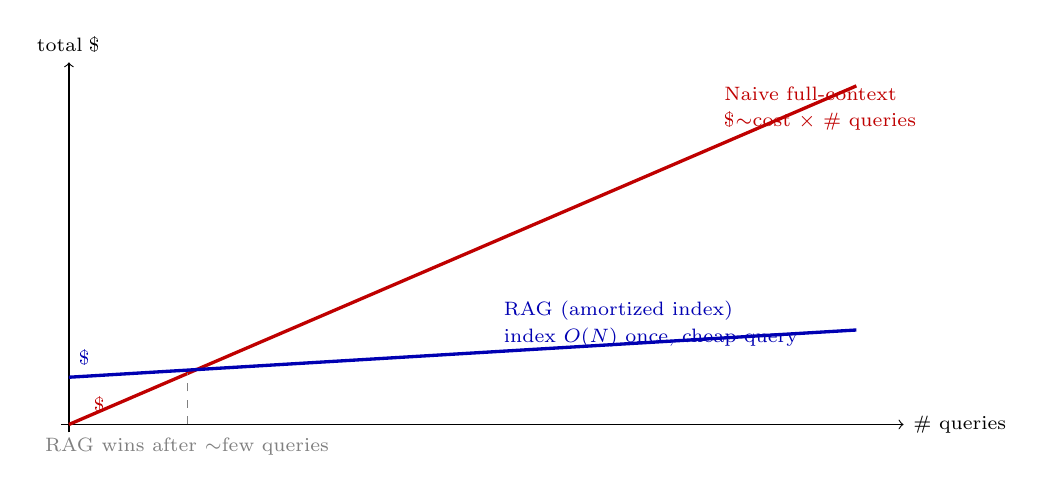
\begin{tikzpicture}[font=\small]
  % axes
  \draw[->] (-0.1,0) -- (10.6,0) node[right, font=\scriptsize] {\# queries};
  \draw[->] (0,-0.1) -- (0,4.6) node[above, font=\scriptsize] {total \$};

  % Naive full-context curve: linear, steep
  \draw[red!75!black, very thick] (0,0.0) -- (10,4.3);
  \node[red!75!black, font=\scriptsize, anchor=west] at (8.2,4.2) {Naive full-context};
  \node[red!75!black, font=\scriptsize, anchor=west] at (8.2,3.85) {\$$\sim$cost $\times$ \# queries};

  % RAG curve: small upfront index cost, very flat query slope
  \draw[blue!70!black, very thick] (0,0.6) -- (10,1.2);
  \node[blue!70!black, font=\scriptsize, anchor=west] at (5.4,1.45) {RAG (amortized index)};
  \node[blue!70!black, font=\scriptsize, anchor=west] at (5.4,1.1) {index $O(N)$ once, cheap query};

  % markers on RAG curve at small \# queries
  \node[blue!70!black, font=\scriptsize] at (0.2,0.85) {\$};
  \node[red!75!black, font=\scriptsize] at (0.4,0.25) {\$};

  % crossover annotation
  \draw[gray, dashed] (1.5,0) -- (1.5,0.65);
  \node[gray, font=\scriptsize, anchor=north] at (1.5,-0.05) {RAG wins after $\sim$few queries};
\end{tikzpicture}
\end{center}

\medskip
\begin{itemize}
\item \textbf{Naive full-context prompting:} cost scales \emph{linearly} with both context size \emph{and} \# queries. Every question repays the full corpus token bill.
\item \textbf{RAG:} pay $O(N)$ embedding calls \emph{once} at index time; each query then ships only the top-$K$ chunks ($\sim$1--5\% of the corpus). Marginal cost per query collapses.
\item \textbf{Callback to Lec.\ 7 T3a (``Tokens, Cost, and Reproducibility''):} per-token API prices and the reproducibility tax come from there. The \emph{RAG-specific} trade-off is: index once, query many; for any project with more than a handful of queries, RAG dominates fine-tuning and naive prompting on total spend \emph{and} latency.
\end{itemize}
\end{frame}

%=============================================================================
\section{Economic Applications}

\begin{frame}{Use Case 1: FOMC Minutes \& Press Conferences}
\begin{itemize}
\item \textbf{Corpus.} The Federal Reserve publishes statements (post-meeting), minutes (3-week lag), press conference transcripts, and (5-year lag) full meeting transcripts. Available 1993--present at \texttt{federalreserve.gov}.

\medskip
\item \textbf{Index pipeline:}
\begin{enumerate}
    \item Scrape PDFs / HTML from the Fed archive.
    \item Parse into speaker turns (minutes) or Q\&A pairs (press conferences).
    \item Chunk with rich metadata: \texttt{meeting\_date}, \texttt{doc\_type}, \texttt{speaker}, \texttt{topic\_section}.
    \item Embed with \texttt{bge-large-en-v1.5}.
    \item Store in Chroma; run BM25 in parallel for hybrid retrieval.
\end{enumerate}

\medskip
\item \textbf{Example research queries:}
\begin{itemize}
    \item \emph{``How did the Committee's framing of inflation expectations evolve from 2021 to 2024?''}
    \item \emph{``Find every appearance of `transitory' in FOMC minutes between 2020 and 2022.''}
    \item \emph{``Which participants most often dissented on rate decisions, 2017--2024?''}
\end{itemize}

\medskip
\item \textbf{Reference:} Hansen, McMahon \& Prat (2018), \emph{QJE}, ``Transparency and Deliberation Within the FOMC: A Computational Linguistics Approach.''
\end{itemize}
\end{frame}

\begin{frame}{Use Case 2: NBER Working Papers}
\begin{itemize}
\item \textbf{Corpus.} $\sim$32{,}000 NBER working papers, 1973--present, available at \texttt{nber.org}. Each has metadata: title, abstract, authors, JEL codes, full PDF.

\medskip
\item \textbf{Use case: literature review automation.} Instead of typing keywords into Google Scholar and reading 50 abstracts, ask:
\begin{quote}
\small\itshape
``Find all NBER working papers from 2019 onwards that estimate the slope of the Phillips curve. Return title, authors, year, the central estimate, and the data source.''
\end{quote}

\medskip
\item \textbf{Pipeline:}
\begin{enumerate}
    \item Index titles + abstracts as one collection (cheap, fast, good for keyword screening).
    \item Index full-paper chunks as a second collection (richer evidence for follow-up questions).
    \item Hybrid retrieval over both. Filter on \texttt{year}, \texttt{JEL\_code}, \texttt{author}.
    \item Generator outputs a structured table from retrieved papers.
\end{enumerate}

\medskip
\item \textbf{Caveat:} Always verify citations against the actual NBER record. Even with RAG, models occasionally garble author lists or year fields.

\medskip
\item \textbf{This is one of the highest-value RAG applications for an active researcher.}
\end{itemize}
\end{frame}

\begin{frame}{Use Case 3: Congressional Record \& Legislative Text}
\begin{itemize}
\item \textbf{Corpus.} The Congressional Record contains every speech delivered on the House and Senate floors since 1873. Daily editions are available at \texttt{congress.gov}.

\medskip
\item \textbf{Use case: tracking how policy debates frame economic issues over time.}
\begin{itemize}
    \item ``How has the rhetoric around `inflation' shifted in House Banking Committee testimony from 2008 to 2024?''
    \item ``Which Senators most frequently cite Federal Reserve research in floor speeches?''
\end{itemize}

\medskip
\item \textbf{The structural challenge.} Congressional Record has a deep hierarchy --- Congress / session / chamber / date / speaker / bill / section. The T2 chunking gotcha applies in full force. A naive chunker that ignores this hierarchy will produce essentially un-citable retrieval results.

\medskip
\item \textbf{Practical fix:} Use a Congress-specific parser (e.g.\ \texttt{congress-api-python}) to extract clean speaker turns with all metadata, then feed those into the chunker.

\medskip
\item \textbf{Reference:} Gentzkow, Shapiro \& Taddy (2019), \emph{Econometrica}, ``Measuring Group Differences in High-Dimensional Choices: Method and Application to Congressional Speech.''
\end{itemize}
\end{frame}

\begin{frame}{Use Case 4: SEC 10-K Filings (Item 1A Risk Factors)}
\begin{itemize}
\item \textbf{Corpus.} EDGAR hosts $\sim$5{,}000{,}000 SEC filings, including the annual 10-K reports of every public US firm. Each 10-K has a standardized ``Item 1A: Risk Factors'' section disclosing material risks.

\medskip
\item \textbf{Use case: cross-firm comparison of disclosed risks.}
\begin{itemize}
    \item \emph{``Compare how the four largest US banks discussed interest-rate risk in their 2022 vs.\ 2023 10-K filings.''}
    \item \emph{``Find all 10-K filings from energy firms in 2024 that mention transition risk from climate policy.''}
\end{itemize}

\medskip
\item \textbf{Pipeline:}
\begin{enumerate}
    \item Use \texttt{sec-edgar-downloader} to pull 10-Ks.
    \item Run a section-aware parser to extract Item 1A only.
    \item Chunk \emph{within} Item 1A, preserving \texttt{cik}, \texttt{ticker}, \texttt{filing\_date}, \texttt{fiscal\_year}.
    \item Store in Chroma. Hybrid retrieval with metadata filter on \texttt{ticker} for cross-firm queries.
\end{enumerate}

\medskip
\item \textbf{References:} Loughran \& McDonald (2011), \emph{JF}, ``When Is a Liability Not a Liability? Textual Analysis, Dictionaries, and 10-Ks.''
Lopez-Lira (2023), \emph{working paper}, ``Risk Factors That Matter.''
\end{itemize}
\end{frame}

\begin{frame}{Use Case 5: Cross-Country Central Bank Speeches}
\begin{itemize}
\item \textbf{Corpus.} The Bank for International Settlements maintains a unified archive of central bank speeches from $\sim$60 institutions, 1997--present, at \texttt{bis.org/cbspeeches}. Other primary sources: ECB, BoE, BoJ, RBA, BoC, RBI, PBoC.

\medskip
\item \textbf{Use case: comparative monetary policy analysis.}
\begin{itemize}
    \item \emph{``How did major central banks frame the post-COVID inflation surge in 2022 speeches? Compare the Fed, ECB, BoE, and BoJ.''}
    \item \emph{``Which central banks most often cite financial-stability concerns alongside inflation, 2010--2024?''}
\end{itemize}

\medskip
\item \textbf{Pipeline notes:}
\begin{itemize}
    \item Add \texttt{country}, \texttt{institution}, \texttt{speaker\_role}, \texttt{language} as metadata.
    \item For non-English speeches, either use a multilingual embedder (\texttt{multilingual-e5-large}) or translate first.
    \item Hybrid retrieval is critical --- many speeches use country-specific institutional jargon a generic embedder won't recognize.
\end{itemize}

\medskip
\item \textbf{This use case is essentially impossible without RAG --- no human can read $\sim$10{,}000 speeches across $\sim$60 institutions per year.}
\end{itemize}
\end{frame}

\begin{frame}{Use Case 6: Combining Structured + Unstructured}
\begin{itemize}
\item RAG isn't only for unstructured text. The most powerful pattern combines a \textbf{structured database} (e.g.\ FRED time series, BEA NIPA tables) with an \textbf{unstructured text store} (Fed speeches, FOMC minutes).

\medskip
\item \textbf{Example query:}
\begin{quote}
\small\itshape
``In months when the unemployment rate fell below 4\%, what did the Fed publicly say about labor markets?''
\end{quote}

\medskip
\item \textbf{Pipeline:}
\begin{enumerate}
    \item \emph{Structured side:} SQL on FRED data. \texttt{SELECT date FROM unrate WHERE value < 4.0;}
    \item \emph{Unstructured side:} retrieve speeches and FOMC minutes whose \texttt{date} falls within those months.
    \item Pass the joined evidence to the LLM with a prompt that says ``summarize how Fed officials characterized the labor market in these specific months.''
\end{enumerate}

\medskip
\item \textbf{This pattern} --- structured SQL filter $\to$ semantic retrieval $\to$ generation --- is uniquely useful for empirical economists. It bridges what economists already know how to do (data) with what they couldn't do before (text at scale).
\end{itemize}
\end{frame}

%=============================================================================
\section{Synthesis}

\begin{frame}{Three-Roles Taxonomy: What Is the RAG Output For? (Callback to Lec.\ 7 T4)}
\small
\begin{center}
\renewcommand{\arraystretch}{1.3}
\begin{tabular}{|p{2.7cm}|p{2.9cm}|p{2.9cm}|p{2.9cm}|}
\hline
\textbf{Use case} & \textbf{Signal} & \textbf{Outcome} & \textbf{Instrument} \\
\hline
FOMC minutes & FOMC stance over time & asset prices, expectations & communication shocks \\
\hline
NBER papers & methodological frontier & citation counts & field-maturity proxy \\
\hline
Congressional Record & policy rhetoric & bill passage, vote share & constituent preferences \\
\hline
SEC 10-K & firm-disclosed risk & stock returns, default & risk-disclosure rule shock \\
\hline
Central-bank speeches & cross-country stance & exchange rates & comparative monetary shock \\
\hline
\end{tabular}
\end{center}

\medskip
\textbf{Reading the table.} RAG returns \emph{evidence}; the econometric role you assign that evidence determines \emph{how you use it}. The same five corpora support \textbf{signal} extraction (text-as-variable), \textbf{outcome} measurement (text-as-target), or \textbf{instrument} construction (text-as-IV). Lec.\ 7 T4 introduced the taxonomy on the LLM side; the same three roles transfer one-to-one to RAG outputs.

\medskip
\textit{Same plumbing, different research design. Pick the role before you write the prompt.}
\end{frame}

\begin{frame}{Synthesis: Three Workflow Patterns}
\begin{enumerate}
\item \textbf{Literature review.} Index a paper repository (NBER, SSRN, RePEc). Query: ``find work on X, summarize, return citations.'' Saves days per project.

\medskip
\item \textbf{Policy-text monitoring over time.} Index an institutional corpus (FOMC, Congress, central banks). Query: ``how did the framing of Y evolve from year A to year B?'' Turns institutional text into a longitudinal research instrument.

\medskip
\item \textbf{Cross-sectional comparative analysis.} Index a corpus where the unit of analysis is a firm or country (10-Ks, central bank speeches). Query: ``compare how entity-1, entity-2, \dots\ discussed Z in year Y.'' Enables cross-firm and cross-country comparisons that were previously infeasible at scale.
\end{enumerate}

\bigskip
\textbf{Methodological punchline.} RAG turns institutional text from \emph{background reading} into a \emph{queryable research instrument}. That is the new capability. Everything else --- chunking, embeddings, vector stores --- is plumbing.
\end{frame}

\begin{frame}{Topic 8.4a Wrap-Up}
\begin{itemize}
\item \textbf{What changed} once we added augmented generation: retrieved chunks become \emph{evidence}, and the generator is forced to cite them. The output is now \emph{auditable}.

\medskip
\item \textbf{When to reach for fine-tuning instead}: style, format, jargon --- not facts. For facts, RAG always wins.

\medskip
\item \textbf{Five corpora, six pipelines}: FOMC, NBER, Congress, SEC 10-K, BIS speeches, structured + unstructured. Same plumbing; different research design.

\medskip
\item \textbf{Methodological move:} institutional text becomes a queryable research instrument. The Section IV synthesis is the take-home.

\medskip
\item \textbf{Up next (Topic 8.4b):} a working OLG demo you can run today, the six common RAG failure modes, evaluation with RAGAS + Cohen's $\kappa$, and the explicit bridge to agentic RAG in Lecture~9.
\end{itemize}
\end{frame}

\end{document}
